\begin{question}
\noindent A space mission designer is scaling up a diagram of a satellite dish component for a museum exhibit. Shape $M$ is enlarged to give shape $M'$, as shown on the grid below.

\begin{center}
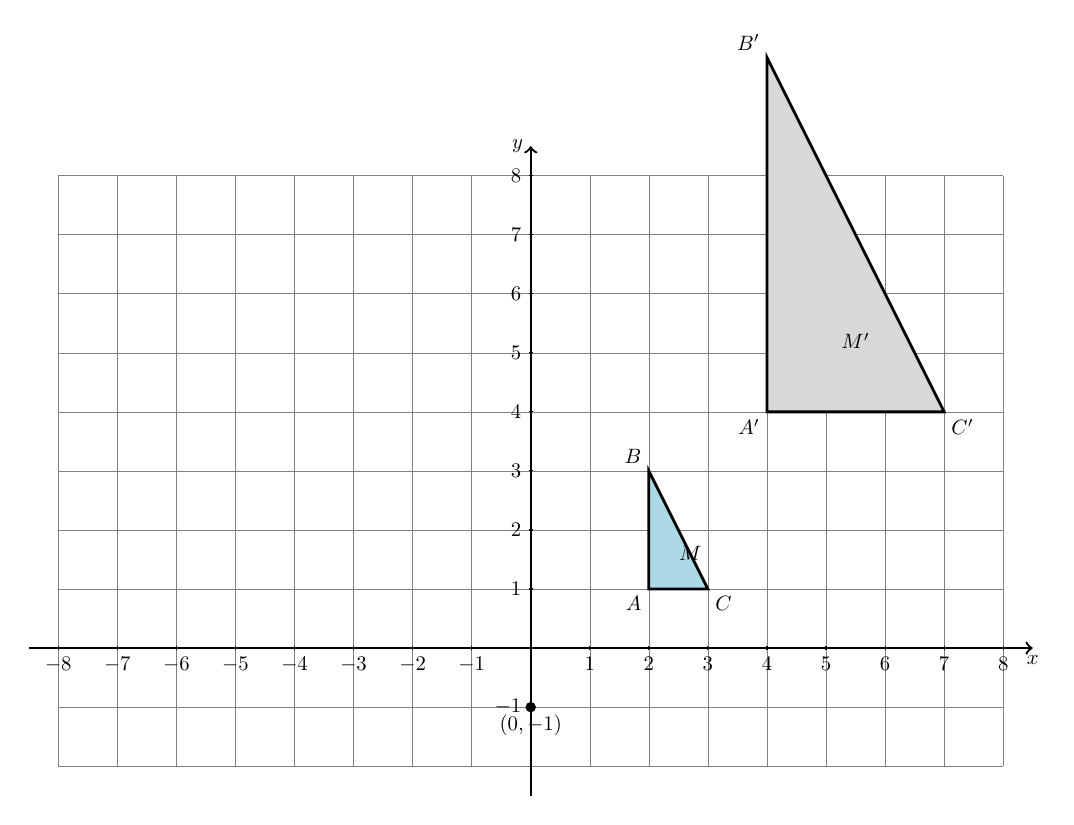
\begin{tikzpicture}[scale=0.75, transform shape]
    \definecolor{borderColour}{HTML}{000000}
    \definecolor{fillColourM}{HTML}{ADD8E6}
    \definecolor{fillColourMprime}{HTML}{D8D8D8}

    \def\axisLimit{8}

    % Draw grid
    \draw[step=1cm,gray,very thin] (-\axisLimit,-2) grid (\axisLimit,\axisLimit);

    % Draw axes
    \draw[thick,->] (-\axisLimit-0.5,0) -- (\axisLimit+0.5,0) node[anchor=north] {$x$};
    \draw[thick,->] (0,-2.5) -- (0,\axisLimit+0.5) node[anchor=east] {$y$};

    % Label x-axis and y-axis
    \foreach \x in {-\axisLimit,...,-1,1,2,...,\axisLimit}
        \draw (\x cm,1pt) -- (\x cm,-1pt) node[anchor=north] {$\x$};
    \foreach \y in {-1,1,2,...,\axisLimit}
        \draw (1pt,\y cm) -- (-1pt,\y cm) node[anchor=east] {$\y$};

    % Shape M: triangle A(2,1), B(2,3), C(3,1)
    \coordinate (A) at (2,1);
    \coordinate (B) at (2,3);
    \coordinate (C) at (3,1);
    \draw[fill=fillColourM, draw=borderColour, line width=1pt] (A) -- (B) -- (C) -- cycle;
    \node[below left] at (A) {$A$};
    \node[above left] at (B) {$B$};
    \node[below right] at (C) {$C$};
    \node at (2.7,1.6) {$M$};

    % Shape M': enlargement scale factor 3 from centre (-2,-2)... but grid must be within limits
    % Centre chosen at (0,-1); vertices: A'(4,4), B'(4,10), C'(7,4)
    \coordinate (Ap) at (4,4);
    \coordinate (Bp) at (4,10);
    \coordinate (Cp) at (7,4);
    \draw[fill=fillColourMprime, draw=borderColour, line width=1pt] (Ap) -- (Bp) -- (Cp) -- cycle;
    \node[below left] at (Ap) {$A'$};
    \node[above left] at (Bp) {$B'$};
    \node[below right] at (Cp) {$C'$};
    \node at (5.5,5.2) {$M'$};

    % centre of enlargement
    \coordinate (O) at (0,-1);
    \fill[black] (O) circle (2.5pt);
    \node[below] at (O) {$(0,-1)$};

\end{tikzpicture}
\end{center}

\noindent Describe fully the single transformation that maps shape $M$ onto shape $M'$.

\vspace{5cm}

\begin{flushright}
    \answerlines{3}{3}
\end{flushright}
\end{question}
